\documentclass[a4paper,12pt]{article}
\usepackage{ctex}
\usepackage{graphicx}
\usepackage{hyperref}
\usepackage{geometry}
\usepackage{xcolor}
\usepackage{listings}
\usepackage{booktabs}
\usepackage{enumitem}
\usepackage{fancyhdr}
\usepackage{float}    % 提供 [H] 选项

\geometry{a4paper,left=2.5cm,right=2.5cm,top=2.5cm,bottom=2.5cm}

\hypersetup{
    colorlinks=true,
    linkcolor=blue,
    filecolor=magenta,      
    urlcolor=cyan,
    pdftitle={系统组用例图说明文档},
    pdfpagemode=FullScreen,
}

\lstset{
    basicstyle=\ttfamily\small,
    breaklines=true,
    frame=single,
    xleftmargin=15pt,
    xrightmargin=15pt,
    backgroundcolor=\color{gray!10}
}

\title{系统组用例图说明文档}
\author{系统组}
\date{\today}

\pagestyle{fancy}
\fancyhf{}
\fancyhead[L]{系统组用例图说明文档}
\fancyhead[R]{\thepage}
\fancyfoot[C]{项目内部文档}

\begin{document}

\maketitle
\tableofcontents
\newpage

\section{文档目的}

本文档通过用例图描述System组在项目中的职责和与其他组(UI组、Data组和Analysis组)的交互关系,明确System组需要提供的功能和服务,为项目各方提供清晰的职责界定和协作指南。

\section{系统组概述}

\subsection{系统组定位}

系统组作为项目的技术基础设施提供者,是项目技术架构的设计者和实现者,负责系统核心功能的开发。系统组的工作直接影响项目的稳定性、可扩展性和技术实现效率。

\subsection{系统组主要职责}

\begin{itemize}
  \item 设计并实现系统整体架构
  \item 构建部署流程
  \item 集成第三方服务
  \item 与Data组协同开发数据库
  \item API设计与实现
  \item 性能优化
  \item 安全保障
  \item 监控与日志系统
\end{itemize}

\section{系统组用例总览}

以下用例图展示了System组的主要职责和与其他组的交互关系:

\begin{figure}[H]
    \centering
    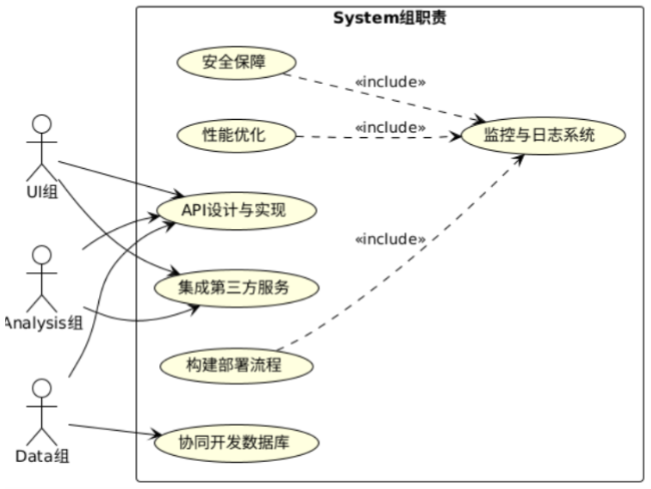
\includegraphics[width=0.75\linewidth]{assets/image2.png}
    \caption{Enter Caption}
    \label{fig:enter-label}
\end{figure}

\section{详细用例说明}

\subsection{构建部署流程}

\begin{figure}[H]
    \centering
    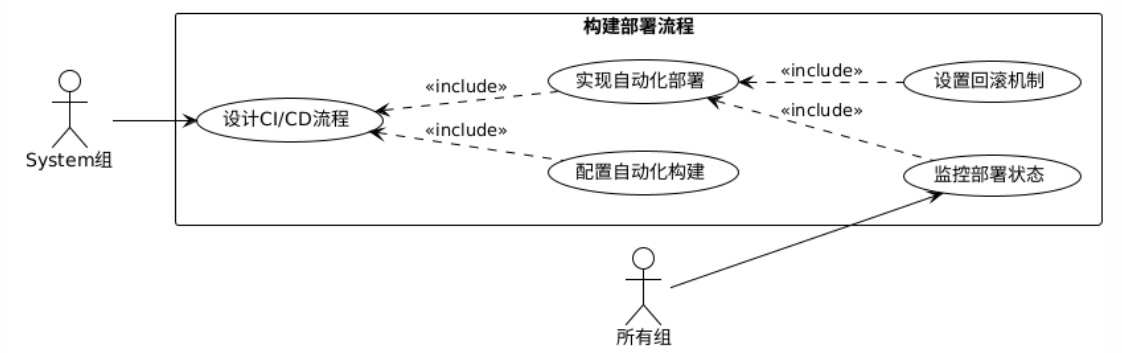
\includegraphics[width=0.75\linewidth]{assets/image1.png}
    \caption{Enter Caption}
    \label{fig:enter-label}
\end{figure}

\textbf{描述}:实现项目代码的自动化构建、测试和部署,提高开发效率和系统稳定性。

\textbf{职责}:
\begin{itemize}
  \item 设计并实现完整的CI/CD流程
  \item 配置自动化构建和测试环境
  \item 提供部署状态监控
  \item 建立部署失败的回滚机制
\end{itemize}

\textbf{与其他组交互}:所有组都会使用部署流程将自己的代码部署到目标环境。

\textbf{交付物}:
\begin{itemize}
  \item CI/CD配置文件
  \item 部署脚本
  \item 部署文档
\end{itemize}

\textbf{包含关系}:此服务包含监控与日志系统的集成,以便追踪部署过程和结果。

\subsection{集成第三方服务(如果其他组需要)}

\begin{figure}[H]
    \centering
    \includegraphics[width=0.75\linewidth]{assets/image.png}
    \caption{Enter Caption}
    \label{fig:enter-label}
\end{figure}

\textbf{描述}:集成项目所需的第三方服务,提供统一的接口供其他组使用。

\textbf{职责}:
\begin{itemize}
  \item 评估和选择适合项目需求的第三方服务
  \item 实现对第三方API的封装
  \item 提供统一的接口规范
  \item 处理第三方服务异常情况
  \item 监控第三方服务的可用性和性能
\end{itemize}

\textbf{与其他组交互}:UI组和Analysis组会使用System组封装的第三方服务接口。

\textbf{交付物}:
\begin{itemize}
  \item 第三方服务集成文档
  \item API封装代码
  \item 服务配置指南
\end{itemize}

\subsection{协同开发数据库}

\begin{figure}
    \centering
    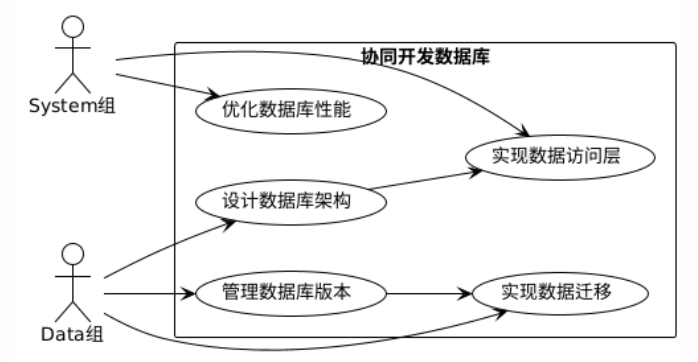
\includegraphics[width=0.75\linewidth]{assets/image8.png}
    \caption{Enter Caption}
    \label{fig:enter-label}
\end{figure}

\textbf{描述}:与Data组协作开发和维护项目数据库系统。

\textbf{职责分工}:
\begin{itemize}
  \item System组:实现数据访问层和数据库性能优化
  \item Data组:负责数据库架构设计、版本管理和数据迁移
\end{itemize}

\textbf{协作方式}:
\begin{itemize}
  \item 共同评审数据库设计方案
  \item 明确各自职责边界
  \item 定期同步开发进展和问题
\end{itemize}

\textbf{交付物}:
\begin{itemize}
  \item 数据库设计文档
  \item 数据库版本控制脚本
  \item 数据访问层代码
\end{itemize}

\subsection{API设计与实现}

\begin{figure}[H]
    \centering
    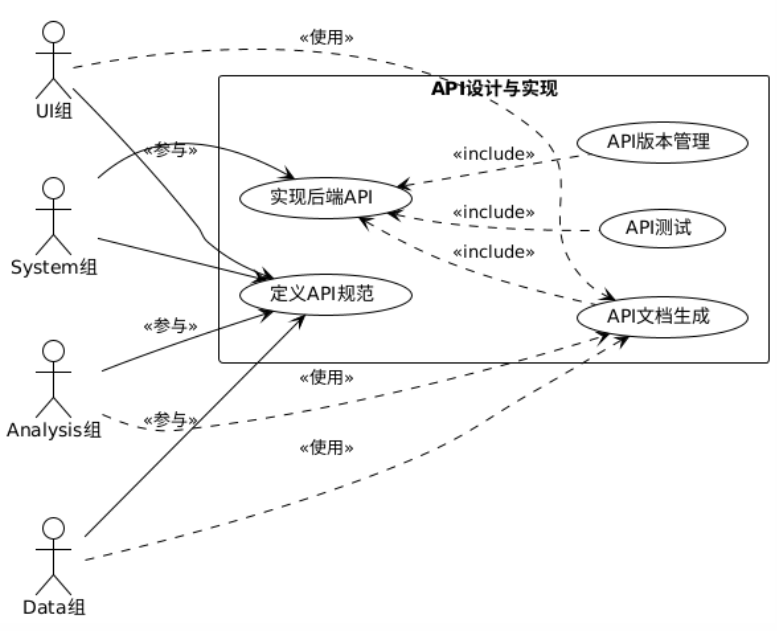
\includegraphics[width=0.75\linewidth]{assets/image4.png}
    \caption{Enter Caption}
    \label{fig:enter-label}
\end{figure}

\textbf{描述}:设计并实现项目所需的所有API接口。

\textbf{职责}:
\begin{itemize}
  \item 制定API设计规范和标准
  \item 实现所有后端API功能
  \item 生成完整的API文档
  \item 进行API单元测试和集成测试
  \item 管理API版本和兼容性
\end{itemize}

\textbf{与其他组交互}:
\begin{itemize}
  \item 其他组参与API规范的讨论和定义
  \item 其他组使用System组提供的API文档进行开发
\end{itemize}

\textbf{交付物}:
\begin{itemize}
  \item API设计文档
  \item API实现代码
  \item API测试用例
  \item Swagger/OpenAPI文档
\end{itemize}

\subsection{性能优化}

\begin{figure}[H]
    \centering
    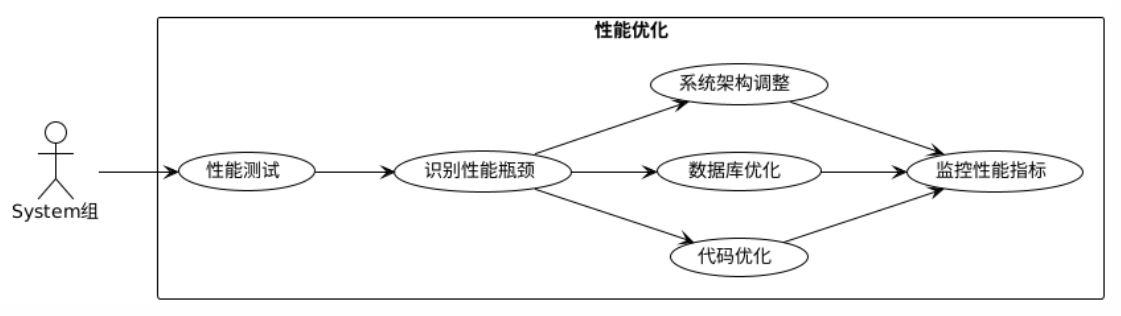
\includegraphics[width=0.75\linewidth]{assets/image5.png}
    \caption{Enter Caption}
    \label{fig:enter-label}
\end{figure}
@enduml


\textbf{描述}:确保系统具有良好的性能和响应速度。

\textbf{职责}:
\begin{itemize}
  \item 设计并执行性能测试方案
  \item 分析并识别系统性能瓶颈
  \item 优化代码实现提高执行效率
  \item 协同Data组进行数据库性能优化
  \item 必要时进行系统架构调整
  \item 持续监控系统性能指标
\end{itemize}

\textbf{交付物}:
\begin{itemize}
  \item 性能分析报告
  \item 优化实施方案
  \item 性能基准测试结果
\end{itemize}

\textbf{包含关系}:此服务包含监控与日志系统,用于收集性能数据和问题诊断。

\subsection{安全保障}

\begin{figure}[H]
    \centering
    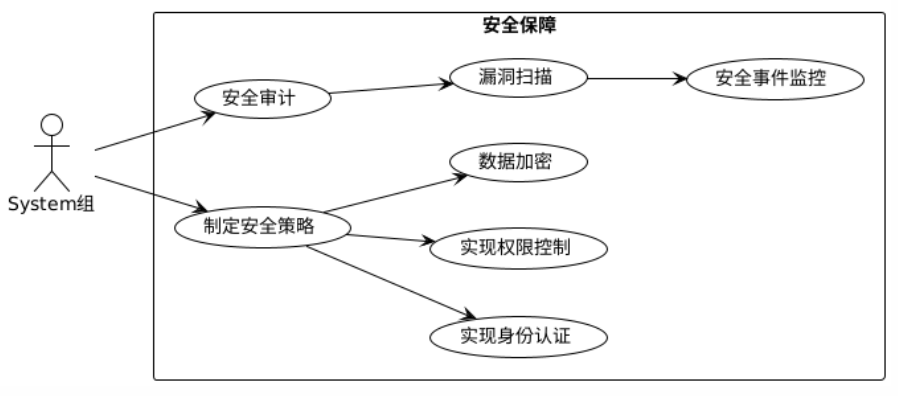
\includegraphics[width=0.75\linewidth]{assets/image6.png}
    \caption{Enter Caption}
    \label{fig:enter-label}
\end{figure}

\textbf{描述}:保障系统和数据的安全性。

\textbf{职责}:
\begin{itemize}
  \item 制定系统安全策略和标准
  \item 实现用户身份认证机制
  \item 实现细粒度的权限控制
  \item 敏感数据加密存储和传输
  \item 定期进行安全审计和漏洞扫描
  \item 实施安全事件监控和响应机制
\end{itemize}

\textbf{交付物}:
\begin{itemize}
  \item 安全策略文档
  \item 安全审计报告
  \item 安全组件与实践指南
\end{itemize}

\textbf{包含关系}:包含监控与日志系统,用于安全事件的检测和响应。

\subsection{监控与日志系统}

\begin{figure}[H]
    \centering
    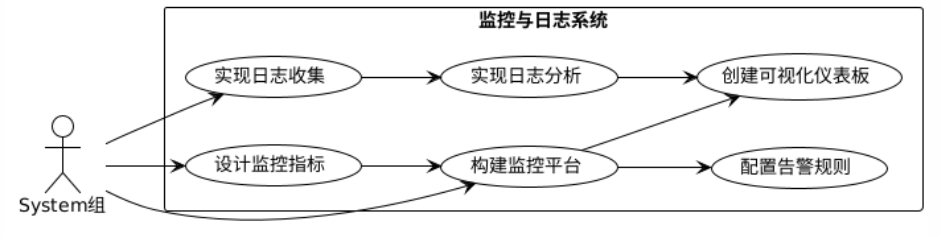
\includegraphics[width=0.75\linewidth]{assets/image7.png}
    \caption{Enter Caption}
    \label{fig:enter-label}
\end{figure}

\textbf{描述}:实时监控系统运行状态,便于问题排查和性能分析。

\textbf{职责}:
\begin{itemize}
  \item 设计系统关键监控指标
  \item 实现全面的日志收集机制
  \item 构建统一的监控平台
  \item 配置合理的告警规则
  \item 实现日志聚合和分析功能
  \item 创建直观的可视化仪表板
\end{itemize}

\textbf{交付物}:
\begin{itemize}
  \item 监控系统配置
  \item 日志分析平台
  \item 告警规则配置
  \item 操作手册
\end{itemize}

\textbf{被其他用例使用}:监控与日志系统被构建部署流程、性能优化和安全保障等多个用例所包含和依赖。

\section{总结}

本文档通过详细的用例图描述了System组在项目中的核心职责,明确了与UI组、Data组和Analysis组的协作界面。System组主要负责系统架构设计、API实现、第三方服务集成等核心技术工作,并与Data组协作开发数据库部分。

通过这些用例图,项目各组成员可以清晰了解System组的工作范围和交付内容,有助于促进团队之间的有效协作。

\section{附录}

\subsection{用例关系说明}

\begin{itemize}
  \item \textbf{包含关系(<<include>>)}:表示一个基础用例被包含在另一个用例中,是必须执行的部分
  \item \textbf{扩展关系(<<extend>>)}:表示一个用例在特定条件下扩展另一个用例的行为
  \item \textbf{使用关系}:表示角色使用某个用例提供的功能
  \item \textbf{参与关系}:表示角色参与某个用例的定义或讨论,但不是主要实施者
\end{itemize}

\subsection{文档修订历史}

\begin{table}[htbp]
\centering
\begin{tabular}{llll}
\toprule
\textbf{版本} & \textbf{日期} & \textbf{修订人} & \textbf{修订内容} \\
\midrule
1.0 & \today & 蔡旭 & 文档初稿 \\
\bottomrule
\end{tabular}
\caption{文档修订历史}
\end{table}

\end{document}
